% ============================================================
%  Shared preamble - matches the Mode-0 / Mode-1 / Mode-2 report house style
% ============================================================
\documentclass[11pt,a4paper]{article}

\usepackage[utf8]{inputenc}
\usepackage[expansion=false]{microtype}
\usepackage[a4paper,left=28mm,right=28mm,top=28mm,bottom=25mm]{geometry}

\usepackage{amsmath,amssymb}
\usepackage{booktabs}
\usepackage{array}
\usepackage{enumitem}
\usepackage{xcolor}
\usepackage{caption}
\usepackage{fancyhdr}
\usepackage{titlesec}
\usepackage{tikz}
\usetikzlibrary{positioning,arrows.meta,calc,fit,backgrounds,shapes.geometric}
\usepackage[most]{tcolorbox}
\usepackage[section]{placeins}
\usepackage[hidelinks]{hyperref}

% ---------- colours ----------
\definecolor{navy}{RGB}{26,60,102}
\definecolor{accent}{RGB}{40,92,148}
\definecolor{softblue}{RGB}{232,240,248}
\definecolor{rulegrey}{RGB}{120,130,140}
\definecolor{orangeacc}{RGB}{196,106,48}
\definecolor{boxblue}{RGB}{219,232,244}
\definecolor{tealbox}{RGB}{214,236,238}
\definecolor{peachbox}{RGB}{250,226,208}
\definecolor{greybox}{RGB}{238,240,242}
\definecolor{greenbox}{RGB}{214,238,214}
\definecolor{pinkbox}{RGB}{250,216,224}
\definecolor{goldbox}{RGB}{250,236,200}

\hypersetup{
  colorlinks=true,
  linkcolor=accent,
  urlcolor=accent,
  citecolor=accent,
  pdftitle={Bluetooth Channel Sounding Mode-3 Combined RTT and Phase-Based Ranging},
  pdfsubject={Formal technical report},
}

% ---------- headings ----------
\titleformat{\section}{\normalfont\Large\bfseries\color{navy}}{\thesection}{0.8em}{}
\titleformat{\subsection}{\normalfont\large\bfseries\color{navy}}{\thesubsection}{0.7em}{}
\titleformat{\subsubsection}{\normalfont\normalsize\bfseries\color{navy}}{\thesubsubsection}{0.6em}{}
\titlespacing*{\section}{0pt}{1.9\baselineskip}{0.8\baselineskip}
\titlespacing*{\subsection}{0pt}{1.2\baselineskip}{0.5\baselineskip}

% ---------- captions ----------
\captionsetup{font=small,labelfont={bf,color=accent},labelsep=colon,width=0.92\textwidth}
\captionsetup[table]{position=above,skip=4pt}
\captionsetup[figure]{position=below,skip=8pt}

% ---------- headers ----------
\pagestyle{fancy}
\fancyhf{}
\renewcommand{\headrulewidth}{0.6pt}
\fancyhead[L]{\small Bluetooth CS Mode-3 Combined RTT and Phase Ranging}
\fancyhead[R]{\small Formal technical report - Revision 1.0}
\fancyfoot[C]{\small\thepage}

% ---------- callout box ----------
\newtcolorbox{callout}[1][]{
  colback=softblue, colframe=accent, boxrule=0.5pt,
  left=6pt,right=6pt,top=5pt,bottom=5pt, arc=1pt,
  fontupper=\small, #1}

% ---------- discrepancy / caution box ----------
\newtcolorbox{caution}[1][]{
  colback=goldbox, colframe=orangeacc, boxrule=0.5pt,
  left=6pt,right=6pt,top=5pt,bottom=5pt, arc=1pt,
  fontupper=\small, #1}

% ---------- table helpers ----------
\newcolumntype{L}[1]{>{\raggedright\arraybackslash}p{#1}}
\renewcommand{\arraystretch}{1.18}

% ---------- macros ----------
\newcommand{\us}{\,\ensuremath{\upmu}s}
\newcommand{\PCT}{\mathrm{PCT}}
\newcommand{\FFO}{\mathrm{FFO}}
\newcommand{\FAE}{\mathrm{FAE}}
\newcommand{\ToF}{\mathrm{ToF}}
\newcommand{\RTT}{\mathrm{RTT}}
\newcommand{\TQI}{\mathrm{TQI}}
\newcommand{\NADM}{\mathrm{NADM}}
\newcommand{\ToD}{\mathrm{ToD}}
\newcommand{\ToA}{\mathrm{ToA}}
\newcommand{\Tsy}{T_{SY}}
\newcommand{\Tgd}{T_{GD}}
\newcommand{\Ttone}{T_{TONE}}
\newcommand{\Tsw}{T_{SW}}
\newcommand{\Tpm}{T_{PM}}
\newcommand{\Trd}{T_{RD}}
\newcommand{\Tipthree}{T_{IP2}}
\newcommand{\Nap}{N_{AP}}
\newcommand{\code}[1]{\texttt{\small #1}}
\providecommand{\upmu}{\mu}

% Core specification citation shorthand
\newcommand{\core}[1]{\textcolor{rulegrey}{\small[Core 6.3, #1]}}

% TikZ block styles reused across figures
\tikzset{
  blk/.style   ={draw=navy!70, fill=softblue, rounded corners=1pt, align=center,
                 font=\scriptsize, inner sep=3.5pt, minimum height=8mm},
  pblk/.style  ={draw=navy!70, fill=white, rounded corners=1pt, align=center,
                 font=\scriptsize, inner sep=3.5pt, minimum height=8mm},
  ar/.style    ={-{Latex[length=2mm]}, draw=navy!80, thick},
  dar/.style   ={-{Latex[length=2mm]}, draw=orangeacc, dashed, thin},
  slot/.style  ={draw=navy!55, font=\scriptsize, align=center, minimum height=7mm},
}

% ============================================================
\begin{document}

% ---------------- Title page ----------------
\thispagestyle{empty}
\vspace*{18mm}
{\color{accent}\small\bfseries FORMAL TECHNICAL REPORT \hfill REVISION 1.0}

\vspace{26mm}
{\raggedright\color{navy}\Huge\bfseries Bluetooth Channel Sounding\par}
\vspace{5mm}
{\raggedright\color{navy}\huge\bfseries Mode-3 Combined Round-Trip Time\\[2mm] and Phase-Based Ranging\par}

\vspace{7mm}
\noindent{\raggedright\color{rulegrey}\large The mirrored sub-slot order, same-step coherence of the
two observables, joint estimation and calibration, per-channel ambiguity resolution, same-step
integrity, and the air-time economics that decide when to use it\par}

\vspace{12mm}
\noindent\rule{\textwidth}{1pt}

\vspace{4mm}
\noindent
This report traces the complete measurement chain of a Bluetooth Channel Sounding Mode-3 step: the
extended packet in which a \code{CS\_SYNC} exchange and a tone exchange share a single step, the
mirrored ordering of the two sub-slots in the initiator and reflector bursts, and the two
observables --- a round-trip time and a set of phase correction terms --- that the step produces
together. It derives the step timing and shows the central structural result: the mirrored order
leaves the phase measurement's reciprocal interval \emph{identical} to Mode-2's while lengthening the
reflector turnaround that governs the round-trip-time clock-scale error, so Mode-3 buys a co-located
round-trip time at a cost paid entirely by the coarse observable that can most easily absorb it. It
develops what same-step acquisition makes newly possible --- per-channel unwrap seeding that is
unconditionally safe across the whole band, joint calibration of loop delay and loop phase on one
hardware path, a joint delay estimator over the combined packet and tone aperture, and a per-channel
integrity check that binds the predictable tone to the unpredictable packet in the same step. A
worked example consistent with the campaign report's configuration quantifies both chains, and the
report closes with an error budget, an air-time trade study, a verification plan, and the boundary
between specified behaviour and implementation choice.

\vfill
\noindent
\begin{tabular}{@{}L{40mm}L{95mm}@{}}
Primary references & Core 6.3, Vol.\ 6, Part H, Sec.\ 4.3.4; Vol.\ 1, Part A, Secs.\ 9.1--9.2 \\
Air-interface timing & Core 6.3, Vol.\ 6, Part H, Secs.\ 4.3 and 4.5 \\
Host interface & Core 6.3, Vol.\ 4, Part E, LE CS Subevent Result event \\
Companion reports & \emph{Mode-0 Frequency Estimation}, Rev.\ 4.0;
                    \emph{Mode-1 RTT Estimation}, Rev.\ 1.0;
                    \emph{Mode-2 Phase-Based Ranging}, Rev.\ 1.0;
                    \emph{Campaign Configuration and Scheduling}, Rev.\ 1.0 \\
Document type & Scientific and implementation-oriented technical report \\
Revision date & 4 September 2026 \\
\end{tabular}

\newpage
\pagenumbering{roman}

% ---------------- Abstract ----------------
\section*{Abstract}
\addcontentsline{toc}{section}{Abstract}

Mode-3 is the combined step mode of Bluetooth Low Energy Channel Sounding
\core{Vol.\ 6, Part H, Sec.\ 4.3.4}. Within one step on one channel, the initiator transmits an
extended packet consisting of a \code{CS\_SYNC} packet, a guard interval, and a tone sequence
covering every antenna path; after the interlude period the reflector transmits the same content in
the \emph{reverse} order, tone sequence first and \code{CS\_SYNC} last. The step therefore yields
both a Mode-1-like round-trip time and a Mode-2-like set of phase correction terms, acquired on the
same channel, through the same hardware path, within a few hundred microseconds of each other.

The estimation theory of the two observables is not new: it is developed in the companion Mode-1 and
Mode-2 reports and applies here unchanged. What is new in Mode-3 is everything that follows from the
two observables being \emph{co-located in one step}, and that is the subject of this report. Four
consequences are developed quantitatively. The mirrored sub-slot order is shown to be a deliberate
optimisation: the reciprocal interval between the two tone measurements is
$\Ttone+\Trd+\Tipthree$, exactly the Mode-2 value, so adding the packets costs the phase chain
nothing, while the reflector turnaround grows to $\Tsy+2\Tgd+2\Ttone+\Trd+\Tipthree$ and makes the
round-trip-time chain roughly two and a half times more sensitive to residual clock-scale error than
Mode-1. A round-trip time available on the \emph{same} channel as each phase sample converts
unwrapping from a fragile sequential accumulation into a set of independent nearest-integer
decisions that remain safe across any gap the 2.4\,GHz band can present. The loop group delay of the
timing chain and the loop phase response of the phase chain are properties of one hardware path
traversed once, so they can be calibrated jointly and checked against each other. And because the
unpredictable \code{CS\_SYNC} and the fully predictable tone occupy the same step, the packet's
integrity metric bounds an attack on the tone in a way that interleaved Mode-1 and Mode-2 steps
cannot.

A worked example at 2\,440\,MHz, using the configuration of the companion campaign report, gives a
step duration of $274\us$, a phase-chain uncertainty of $1.57$\,cm and a timing-chain uncertainty of
$12.8$\,cm, and yields a $3\sigma$ cross-observable consistency gate of $39$\,cm. An air-time study
shows Mode-3 to be $23.7\%$ cheaper in occupancy than a Mode-1 and a Mode-2 step taken separately,
but $16.6\%$ more expensive than the sparse-sub-mode campaign pattern it would replace.

\begin{callout}
\textbf{Status and interpretation.} Normative claims are tied to the cited Bluetooth Core
Specification sections. Estimators, joint-estimation formulations, calibration schemes, quality
metrics and aggregation rules are representative implementation methods. Timing parameter value
lists and report field encodings should be read from the adopted specification revision in force;
where this report states them, they are given to make the equations concrete, and section numbering
within Volume 6, Part H has changed between Core revisions. Two internal inconsistencies in the
existing report series that this document had to resolve are flagged explicitly in
Section~\ref{sec:discrepancies}. The Bluetooth specification and adopted test specifications remain
authoritative for conformance.
\end{callout}

\newpage
\tableofcontents
\newpage
\pagenumbering{arabic}
\setcounter{page}{1}

% ============================================================
\section{Scope and measurement objective}
% ============================================================

Bluetooth Channel Sounding uses four step modes, defined in Core 6.3, Volume 6, Part H,
Sections 4.3.1--4.3.4. Mode-0 establishes the relative frequency and timing scale between the two
devices. Mode-1 uses that scale to measure a round-trip time. Mode-2 measures phase on tone
exchanges. Mode-3 performs both measurements within a single step.

The Mode-3 measurement objective is the union of the Mode-1 and Mode-2 objectives, with one addition
that is easy to overlook and is the reason the mode exists: the two observables carry a
\emph{binding} to each other. Per step, the reported set is

\begin{itemize}[leftmargin=1.4em,itemsep=1pt]
  \item the initiator's and reflector's timing differences, from which a round-trip time is formed
        exactly as in Mode-1 \core{Vol.\ 4, Part E, LE CS Subevent Result};
  \item the per-antenna-path phase correction terms and tone quality indicators from both devices,
        from which a two-way phase is formed exactly as in Mode-2; and
  \item the fact, guaranteed by the step structure rather than by inference, that both were measured
        on the same channel, through the same antenna path and gain state, within one step.
\end{itemize}

\subsection{What this report does and does not repeat}

The estimation theory of each observable in isolation is developed in the companion reports and is
not reproduced here. Time-of-arrival estimation from a \code{CS\_SYNC} packet --- matched filtering,
sub-sample interpolation, maximum likelihood, group-delay regression, first-path detection under
multipath, and the Cram\'er--Rao bound relating timing variance to root-mean-square bandwidth and
accumulated signal-to-noise ratio --- is the subject of the Mode-1 report. Per-slot phase estimation
and the conversion of a set of per-channel phase correction terms into a distance --- coherent
averaging, frequency estimation, front-end impairments, slope regression, inverse-transform channel
impulse response formation, super-resolution and ambiguity --- is the subject of the Mode-2 report.
Both apply to Mode-3 without modification.

This report covers what is specific to Mode-3: the step structure and its timing consequences
(Sections~\ref{sec:timing}--\ref{sec:mirror}), what same-step acquisition makes newly possible
(Sections~\ref{sec:shared}--\ref{sec:joint}), the combined error budget and the cross-observable
consistency gate (Sections~\ref{sec:precision} and~\ref{sec:example}), same-step integrity
(Section~\ref{sec:security}), and the air-time economics that decide whether to configure Mode-3 at
all (Section~\ref{sec:economics}).

\begin{callout}
\textbf{Three properties that are frequently confused.} (1) Mode-3 is \emph{not} simply a Mode-1 step
and a Mode-2 step concatenated: the sub-slot order is mirrored between the two devices, and that
mirroring is what keeps the phase chain's reciprocal interval as short as Mode-2's. (2) Mode-3 does
not improve either observable's precision --- a Mode-3 round-trip time is no better than a Mode-1
round-trip time on the same configuration, and its phase samples are no better than Mode-2's. What
improves is everything that depends on the two being \emph{jointly} available. (3) Mode-3 is not
free: its step is longer than either constituent, and whether it is cheaper than the alternative
depends entirely on how often the campaign would otherwise schedule a round-trip-time step.
\end{callout}
% ============================================================
\section{Normative framework and terminology}
% ============================================================

\begin{table}[h]
\caption{Normative map for the Mode-3 combined measurement. Section numbering should be confirmed
against the specification revision in force.}
\label{tab:normmap}
\centering\small
\begin{tabular}{@{}L{42mm}L{51mm}L{51mm}@{}}
\toprule
Source & What it defines & Question answered \\
\midrule
Core 6.3, Vol.\ 1, Part A, Sec.\ 9.1 & CS procedure architecture; ordering of calibration and ranging steps & Why must Mode-0 precede Mode-3? \\
Core 6.3, Vol.\ 1, Part A, Sec.\ 9.2 & Distance estimation from phase and amplitude information & What is the intended use of the phase observable? \\
Core 6.3, Vol.\ 6, Part H, Sec.\ 4.3.4 & Mode-3 step structure: the extended packet and its sub-slot order in each direction & What is transmitted, in which order, and when? \\
Core 6.3, Vol.\ 6, Part H, Sec.\ 4.3.2 & Mode-1 step, whose packet exchange Mode-3 embeds & How is the round-trip time formed? \\
Core 6.3, Vol.\ 6, Part H, Sec.\ 4.3.3 & Mode-2 step, whose tone exchange Mode-3 embeds & How is the phase observable formed? \\
Core 6.3, Vol.\ 6, Part H, Sec.\ 4.3 & $\Tsy$, $\Tgd$, $\Tsw$, $\Tpm$, $\Trd$, interlude and $T_{FCS}$ value sets & Which step timings may be configured? \\
Core 6.3, Vol.\ 6, Part H, Sec.\ 4.4 & \code{CS\_SYNC} construction: access address, trailer, sounding and random sequences & What waveform is the timing receiver matched to? \\
Core 6.3, Vol.\ 6, Part H, Sec.\ 4.5 & Antenna path handling, permutation, tone extension slot & Which physical path does a tone slot correspond to? \\
Core 6.3, Vol.\ 6, Part A, Sec.\ 3.5 & Frequency measurement and generation in CS & On what carrier are the packet and tone expected? \\
Core 6.3, Vol.\ 4, Part E, LE CS Subevent Result event & Per-step timing, $\PCT$, $\TQI$ and $\NADM$ reporting & How is the measurement exposed to the host? \\
RFPHY.TS / LL.TS, CS step Mode-3 clauses & Instrument-level verification of the combined step & How is the behaviour tested? \\
\bottomrule
\end{tabular}
\end{table}

\begin{table}[h]
\caption{Principal symbols. Symbols shared with the companion reports keep their meaning.}
\label{tab:symbols}
\centering\small
\begin{tabular}{@{}L{28mm}L{78mm}L{22mm}@{}}
\toprule
Symbol & Meaning & Units \\
\midrule
$\Tsy$ & \code{CS\_SYNC} packet duration & s \\
$\Tgd$ & Guard interval between \code{CS\_SYNC} and tone sequence & s \\
$\Ttone$ & Tone-sequence duration, $(\Tsw+\Tpm)(\Nap+1)$ & s \\
$\Tsw,\ \Tpm$ & Antenna path switch and phase measurement periods & s \\
$\Trd$ & Transmitter ramp-down period & s \\
$T_{IP2}$ & Interlude period for Mode-3 \core{Vol.\ 6, Part H, Sec.\ 4.3.4} & s \\
$\Nap$ & Number of antenna paths & --- \\
$\Delta T$ & Interval between the reciprocal tone measurements of one path & s \\
$B_R$ & Reflector turnaround interval, \code{CS\_SYNC} arrival to departure & s \\
$A_I$ & Initiator-measured round interval $\ToA_I-\ToD_I$ & s \\
$\RTT,\ \ToF$ & Round-trip time and one-way time of flight & s \\
$\Theta(f_k)$ & Two-way phase sum on channel $k$ & rad \\
$H[k]$ & Assembled frequency-domain channel estimate & --- \\
$D_{loop}$ & Total calibrated loop group delay of the four chains & s \\
$\Phi_{loop}(f)$ & Total calibrated loop phase response & rad \\
$\epsilon$ & Residual fractional frequency offset after Mode-0 & --- \\
$\hat d_{\RTT},\ \hat d_{\Theta}$ & Range from the timing and phase chains & m \\
$\TQI,\ \NADM$ & Tone quality indicator; Normalized Attack Detector Metric & index \\
\bottomrule
\end{tabular}
\end{table}

% ============================================================
\section{Two inconsistencies in the series, and how this report resolves them}
\label{sec:discrepancies}
% ============================================================

Two points had to be settled before the timing algebra of Section~\ref{sec:timing} could be written,
because the existing material in this series disagrees with itself. Both are recorded here rather
than buried, because both affect numbers that other documents depend on.

\begin{callout}
\textbf{(1) The interlude is $T_{IP2}$ --- resolved.} This was an open question when this report was
first drafted: the Mode-3 timing artwork labelled the interlude $T_{IP,2}$ while the companion campaign
report used $T_{IP1}$. Core 6.3 settles it. Table 4.10 of the Channel Sounding part gives the Mode-3
step as $\Tsy+\Tgd+(\Tsw+\Tpm)(\Nap+1)$, $\Trd$, $\mathbf{T_{IP2}}$,
$(\Tsw+\Tpm)(\Nap+1)+\Tgd+\Tsy$, $\Trd$ \core{Vol.\ 6, Part H, Sec.\ 4.3.4}, and the accompanying
text states that ``the duration of $T_{IP2}$ is defined in Section 4.3.3''. The artwork is correct and
the campaign report is wrong. Since $T_{IP1}$ and $T_{IP2}$ share the value set
$\{10,20,30,40,50,60,80,145\}\us$, no number in this report changes; only the parameter an
implementation must read does. This report writes the interlude as $\Tipthree$ throughout.
\end{callout}

\begin{caution}
\textbf{(2) The guard intervals are missing from the campaign report's step duration.} The campaign
report gives
\[
T_{step,3} \;=\; 2\Tsy + 2(\Tsw+\Tpm)(\Nap+1) + 2\Trd + T_{IP1},
\]
which omits the guard interval $\Tgd$ that separates the \code{CS\_SYNC} packet from the tone
sequence in \emph{each} of the two bursts. With the series' fixed $\Tgd = 10\us$, the omission
understates every Mode-3 step by $2\Tgd = 20\us$. For the campaign report's own configuration this is
$254\us$ against a correct $274\us$, an error of $7.9\%$ in step duration that propagates into
subevent occupancy, steps per subevent and radio duty cycle.

\emph{Confirmed against the specification.} Core 6.3 Table 4.10 shows the guard interval explicitly
in \emph{both} extended packets \core{Vol.\ 6, Part H, Sec.\ 4.3.4}, and Section 2.6 fixes
$\Tgd = 10\us$ ``independent of the LE PHY being used''. This report uses
Eq.~\eqref{eq:stepdur}, which includes both. The campaign report should be corrected if its Mode-3
numbers are relied upon for scheduling.
\end{caution}

% ============================================================
\section{Position of Mode-3 in the CS subevent}
% ============================================================

Figure~\ref{fig:stack} places Mode-3 in the causal chain. Mode-0 still runs first and still supplies
the subevent frequency reference $\FFO^{*}_{RX}$, which Mode-3 needs for three separate purposes:
carrier placement for both the packet and the tone, rescaling of the reflector's reported turnaround
interval in the timing chain, and bounding of the drift term in the phase chain
\core{Vol.\ 6, Part H, Sec.\ 4.3.1; Vol.\ 6, Part A, Sec.\ 3.5}.

\begin{figure}[h]
\centering
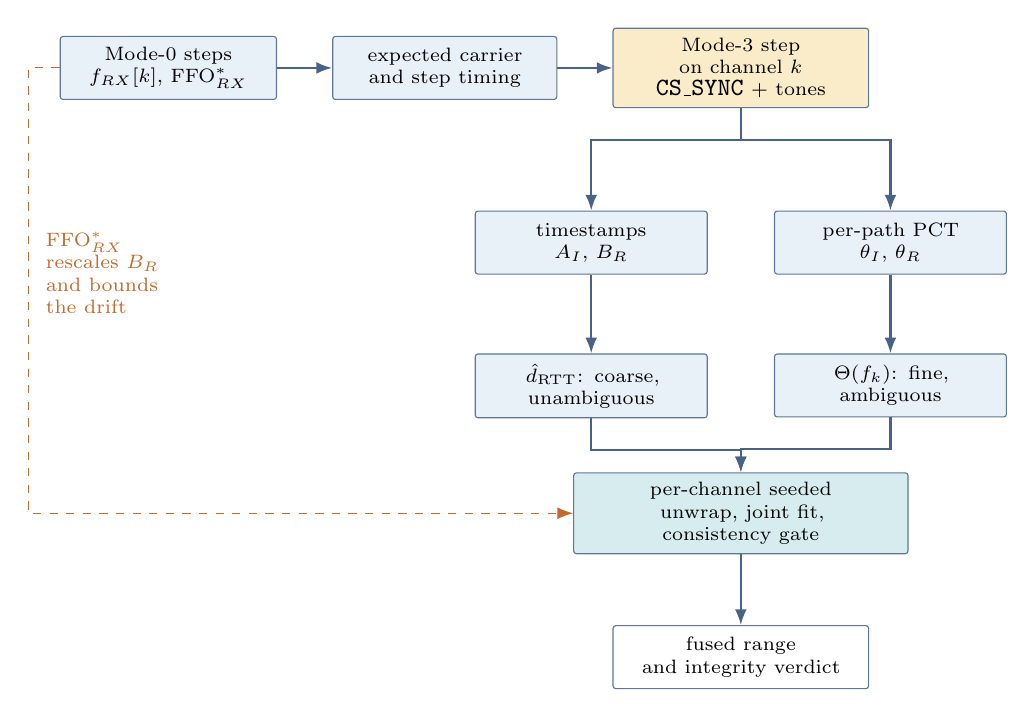
\begin{tikzpicture}[node distance=6mm and 7mm]
\node[blk,text width=25mm] (m0) {Mode-0 steps\\ $f_{RX}[k]$, $\FFO^{*}_{RX}$};
\node[blk,right=of m0,text width=26mm] (carr) {expected carrier\\ and step timing};
\node[blk,right=of carr,text width=30mm,fill=goldbox] (m3) {Mode-3 step on channel $k$\\ \code{CS\_SYNC} + tones};

\node[blk,below=13mm of m3,text width=27mm,xshift=-19mm] (ts) {timestamps\\ $A_I$, $B_R$};
\node[blk,below=13mm of m3,text width=27mm,xshift=19mm] (pct) {per-path $\PCT$\\ $\theta_I$, $\theta_R$};

\node[blk,below=10mm of ts,text width=27mm] (rtt) {$\hat d_{\RTT}$: coarse,\\ unambiguous};
\node[blk,below=10mm of pct,text width=27mm] (theta) {$\Theta(f_k)$: fine,\\ ambiguous};

\node[blk,below=11mm of $(rtt)!0.5!(theta)$,text width=40mm,fill=tealbox] (fuse)
  {per-channel seeded unwrap, joint fit,\\ consistency gate};
\node[pblk,below=9mm of fuse,text width=30mm] (out) {fused range\\ and integrity verdict};

\draw[ar] (m0)--(carr); \draw[ar] (carr)--(m3);
\draw[ar] (m3.south) -- ++(0,-4mm) -| (ts.north);
\draw[ar] (m3.south) -- ++(0,-4mm) -| (pct.north);
\draw[ar] (ts)--(rtt); \draw[ar] (pct)--(theta);
\draw[ar] (rtt.south) -- ++(0,-4mm) -| (fuse.north);
\draw[ar] (theta.south) -- ++(0,-4mm) -| (fuse.north);
\draw[ar] (fuse)--(out);
\draw[dar] (m0.west) -- ++(-4mm,0) |- ($(fuse.west)+(-6mm,0)$) -- (fuse.west);
\node[font=\scriptsize,color=orangeacc,anchor=west,align=left] at ($(m0.west)+(-3mm,-26mm)$)
  {$\FFO^{*}_{RX}$\\ rescales $B_R$\\ and bounds\\ the drift};
\end{tikzpicture}
\caption{Position of Mode-3. A single step forks into the timing and phase chains, which rejoin at a
fusion stage that is now \emph{per channel} rather than per procedure, because both observables were
acquired on the same channel in the same step.}
\label{fig:stack}
\end{figure}

The structural difference from a campaign that interleaves Mode-1 and Mode-2 steps is visible in the
figure: the two chains diverge and reconverge \emph{within one channel}. In an interleaved campaign
the reconvergence happens only at the procedure level, after aggregation, because the round-trip time
was measured on a different channel at a different time.

% ============================================================
\section{Mode-3 step structure and timing}
\label{sec:timing}
% ============================================================

\subsection{The extended packet and its mirrored order}

A Mode-3 step carries an \emph{extended packet} in each direction
\core{Vol.\ 6, Part H, Sec.\ 4.3.4}. The initiator's extended packet is a \code{CS\_SYNC} packet,
then a guard interval, then a tone sequence covering every antenna path. The reflector's extended
packet contains the same three elements in the reverse order: tone sequence, guard interval,
\code{CS\_SYNC}. Both are transmitted on the same channel, and each is followed by the transmitter
ramp-down period.

\begin{figure}[h]
\centering
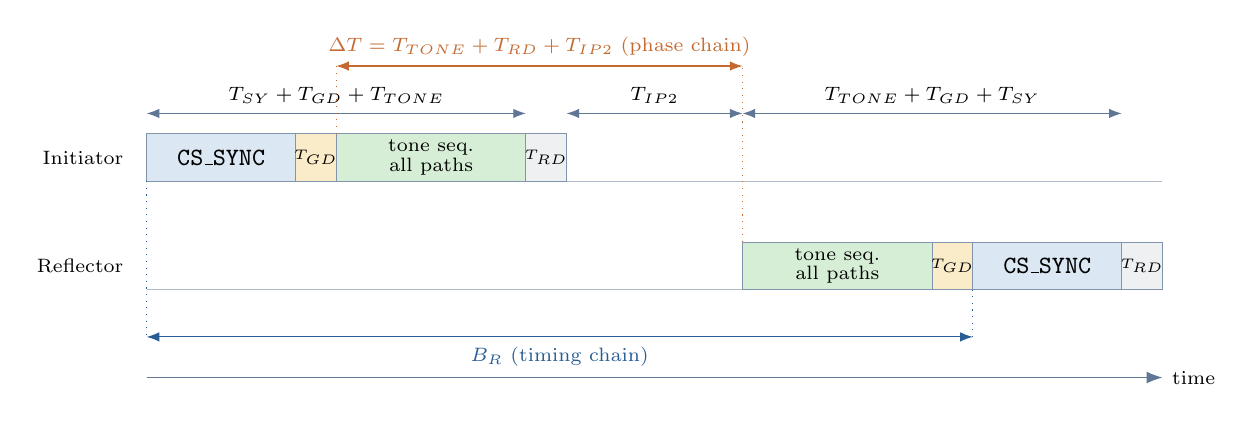
\begin{tikzpicture}[x=0.86mm,y=0.86mm]
\def\yI{16} \def\yR{0}
\draw[-{Latex[length=2mm]},draw=navy!70] (0,\yR-13) -- (150,\yR-13) node[right,font=\scriptsize] {time};
\node[font=\scriptsize,anchor=east] at (-2,\yI+3.5) {Initiator};
\node[font=\scriptsize,anchor=east] at (-2,\yR+3.5) {Reflector};
\draw[draw=navy!35] (0,\yI) -- (150,\yI);
\draw[draw=navy!35] (0,\yR) -- (150,\yR);

% initiator extended packet: SYNC | GD | TONE | RD
\draw[slot,fill=boxblue] (0,\yI)  rectangle (22,\yI+7) node[midway] {\code{CS\_SYNC}};
\draw[slot,fill=goldbox] (22,\yI) rectangle (28,\yI+7) node[midway,font=\tiny] {$\Tgd$};
\draw[slot,fill=greenbox](28,\yI) rectangle (56,\yI+7) node[midway,align=center] {tone seq.\\[-1pt] all paths};
\draw[slot,fill=greybox] (56,\yI) rectangle (62,\yI+7) node[midway,font=\tiny] {$\Trd$};

% reflector extended packet: TONE | GD | SYNC | RD
\draw[slot,fill=greenbox](88,\yR) rectangle (116,\yR+7) node[midway,align=center] {tone seq.\\[-1pt] all paths};
\draw[slot,fill=goldbox](116,\yR) rectangle (122,\yR+7) node[midway,font=\tiny] {$\Tgd$};
\draw[slot,fill=boxblue](122,\yR) rectangle (144,\yR+7) node[midway] {\code{CS\_SYNC}};
\draw[slot,fill=greybox](144,\yR) rectangle (150,\yR+7) node[midway,font=\tiny] {$\Trd$};

% interlude bracket
\draw[{Latex[length=1.6mm]}-{Latex[length=1.6mm]},draw=navy!70] (62,\yI+10) -- (88,\yI+10)
   node[midway,above,font=\scriptsize] {$\Tipthree$};
\draw[{Latex[length=1.6mm]}-{Latex[length=1.6mm]},draw=navy!70] (0,\yI+10) -- (56,\yI+10)
   node[midway,above,font=\scriptsize] {$\Tsy+\Tgd+\Ttone$};
\draw[{Latex[length=1.6mm]}-{Latex[length=1.6mm]},draw=navy!70] (88,\yI+10) -- (144,\yI+10)
   node[midway,above,font=\scriptsize] {$\Ttone+\Tgd+\Tsy$};

% phase reciprocal interval: tone start to tone start
\draw[{Latex[length=1.6mm]}-{Latex[length=1.6mm]},draw=orangeacc] (28,\yI+17) -- (88,\yI+17)
   node[midway,above,font=\scriptsize,color=orangeacc] {$\Delta T=\Ttone+\Trd+\Tipthree$ (phase chain)};
\draw[dotted,draw=orangeacc] (28,\yI+7) -- (28,\yI+17);
\draw[dotted,draw=orangeacc] (88,\yR+7) -- (88,\yI+17);

% RTT turnaround: SYNC start to SYNC start
\draw[{Latex[length=1.6mm]}-{Latex[length=1.6mm]},draw=accent] (0,\yR-7) -- (122,\yR-7)
   node[midway,below,font=\scriptsize,color=accent] {$B_R$ (timing chain)};
\draw[dotted,draw=accent] (0,\yI) -- (0,\yR-7);
\draw[dotted,draw=accent] (122,\yR) -- (122,\yR-7);
\end{tikzpicture}
\caption{Mode-3 step. The initiator sends \code{CS\_SYNC}, guard, tone sequence; the reflector sends
tone sequence, guard, \code{CS\_SYNC}. The mirrored order places the two tone sequences \emph{adjacent
across the interlude}, so the phase chain's reciprocal interval $\Delta T$ is as short as it is in a
pure Mode-2 step, while the two \code{CS\_SYNC} packets are pushed to the outer edges, lengthening
the reflector turnaround $B_R$ seen by the timing chain.}
\label{fig:m3timing}
\end{figure}

\subsection{Step duration and the two derived intervals}

Writing $\Ttone = (\Tsw+\Tpm)(\Nap+1)$ for the tone-sequence duration
\core{Vol.\ 6, Part H, Secs.\ 4.3.3 and 4.5}, the nominal step duration is
\begin{equation}
T_{step,3} \;=\; 2\bigl[\Tsy + \Tgd + \Ttone + \Trd\bigr] \;+\; \Tipthree ,
\label{eq:stepdur}
\end{equation}
with the frequency-change period $T_{FCS}$ inserted between scheduled steps that use different
channels \core{Vol.\ 6, Part H, Sec.\ 4.3}. Two further intervals, neither of which is $T_{step,3}$,
govern the two error chains.

The phase chain is governed by the interval between the reflector's measurement of the initiator's
tone on antenna path $p$ and the initiator's measurement of the reflector's tone on the same path.
The initiator's slot $p$ begins at $\Tsy+\Tgd+(p-1)(\Tsw+\Tpm)$; the reflector's burst begins at
$\Tsy+\Tgd+\Ttone+\Trd+\Tipthree$ and its slot $p$ begins $(p-1)(\Tsw+\Tpm)$ later. Subtracting,
\begin{equation}
\Delta T \;=\; \Ttone \;+\; \Trd \;+\; \Tipthree ,
\label{eq:deltaT}
\end{equation}
independent of $p$, and of $\Tsy$ and $\Tgd$.

The timing chain is governed by the reflector turnaround, from the arrival of the initiator's
\code{CS\_SYNC} to the departure of its own. Reading Figure~\ref{fig:m3timing},
\begin{equation}
B_R \;=\; \Tsy \;+\; 2\Tgd \;+\; 2\Ttone \;+\; \Trd \;+\; \Tipthree .
\label{eq:BR}
\end{equation}

\begin{table}[h]
\caption{Mode-3 timing parameters. Permitted sets are configuration-dependent and subject to both
devices' declared capabilities; read the value lists from the specification revision in force
\core{Vol.\ 6, Part H, Sec.\ 4.3; Vol.\ 4, Part E, CS configuration}. The three fixed values are
those used consistently across this report series.}
\label{tab:timing}
\centering\small
\begin{tabular}{@{}L{18mm}L{54mm}L{56mm}@{}}
\toprule
Parameter & Meaning & Representative permitted values \\
\midrule
$\Tsy$    & \code{CS\_SYNC} packet duration & PHY- and RTT-type-dependent; LE 2M: 26, 42, 58, 74, 90\us \\
$\Tgd$    & Guard interval between \code{CS\_SYNC} and tone sequence & 10\us (fixed in this series) \\
$\Tsw$    & Antenna path switch period, including RF and phase settling & 1, 2, 4, 10\us when switching is performed; 0 with a single antenna \\
$\Tpm$    & Phase measurement period & 10, 20, 40\us ($40\us$ mandatory) \\
$\Trd$    & Transmitter ramp-down & 5\us (fixed) \\
$T_{IP2}$ & Interlude period, confirmed for Mode-3 (\S\ref{sec:discrepancies}) & 10, 20, 30, 40, 50, 60, 80, 145\us ($145\us$ mandatory) \\
$T_{FCS}$ & Frequency-change period between steps & 15, 20, 30, 40, 50, 60, 80, 100, 120, 150\us \\
\bottomrule
\end{tabular}
\end{table}

\begin{table}[h]
\caption{Step duration, phase reciprocal interval and reflector turnaround from
Eqs.~\eqref{eq:stepdur}--\eqref{eq:BR}, with $\Tgd=10\us$, $\Trd=5\us$ and the LE 2M PHY. The
Mode-1 and Mode-2 columns use the companion reports' formulas at the same settings.}
\label{tab:durations}
\centering\small
\begin{tabular}{@{}rrrrr@{\hspace{7mm}}rrr@{}}
\toprule
$\Tsy$ & $\Nap$ & $\Tsw$ & $\Tpm$ & $\Tipthree$ & $T_{step,3}$ & $\Delta T$ & $B_R$ \\
\midrule
42 & 4 & 2  & 10 & 40  & $274\us$ & $105\us$ & $227\us$ \\
42 & 1 & 2  & 10 & 40  & $202\us$ & $69\us$  & $155\us$ \\
42 & 4 & 2  & 10 & 145 & $379\us$ & $210\us$ & $332\us$ \\
74 & 4 & 2  & 10 & 40  & $338\us$ & $105\us$ & $259\us$ \\
42 & 4 & 10 & 20 & 40  & $454\us$ & $195\us$ & $407\us$ \\
42 & 4 & 2  & 10 & 10  & $244\us$ & $75\us$  & $197\us$ \\
\bottomrule
\end{tabular}
\end{table}

Reading the table against Eqs.~\eqref{eq:deltaT} and~\eqref{eq:BR} shows how differently the two
chains respond to configuration. Lengthening the \code{CS\_SYNC} packet from 42 to $74\us$ --- moving
from a 32-bit to a 96-bit sounding sequence --- improves the timing chain's thermal precision by
$\sqrt{3}$ and leaves $\Delta T$ untouched, so it is close to free for the phase chain. Enlarging the
tone sequence, by contrast, lengthens \emph{both} $\Delta T$ and $B_R$, and does so twice over in the
latter.
% ============================================================
\section{Why the sub-slot order is mirrored}
\label{sec:mirror}
% ============================================================

The mirroring of the two extended packets is the single design decision that distinguishes Mode-3
from a naive concatenation of a Mode-1 and a Mode-2 step, and it is worth deriving rather than
asserting.

\subsection{The counterfactual}

Suppose both devices transmitted \code{CS\_SYNC} first and the tone sequence second. Repeating the
arithmetic of Section~\ref{sec:timing} for that hypothetical ordering,
\begin{equation}
\Delta T^{(\text{un-mirr.})} \;=\; B_R^{(\text{un-mirr.})}
   \;=\; \Tsy + \Tgd + \Ttone + \Trd + \Tipthree ,
\label{eq:unmirrored}
\end{equation}
so the two intervals would be equal. Mirroring shortens the first by $\Tsy+\Tgd$ and lengthens the
second by $\Tgd+\Ttone$. For the configuration of Section~\ref{sec:example} this moves
$\Delta T$ from $157\us$ to $105\us$, a reduction of $33\%$, and $B_R$ from $157\us$ to $227\us$, an
increase of $45\%$.

\subsection{Why that is the right trade}

Both intervals enter their respective chains through the same physical mechanism --- a residual
fractional frequency offset $\epsilon$ integrated over an interval --- and with the same
coefficient. From the companion reports, the phase chain acquires a bias
$c\,\epsilon\,\Delta T/2$ (Mode-2 report, Eq.\ for $\delta d_\epsilon$) and the timing chain acquires
a bias $c\,\epsilon\,B_R/2$ (Mode-1 report, clock-scale correction). The two are numerically
identical functions of their intervals. What differs is the \emph{budget each is spent against}.

\begin{table}[h]
\caption{Effect of the mirrored ordering on the residual-frequency bias in each chain, for the
worked configuration of Section~\ref{sec:example}. The final columns express each change as a
fraction of that chain's total uncertainty from Table~\ref{tab:example}: $15.7$\,mm for the phase
chain and $128$\,mm for the timing chain.}
\label{tab:mirror}
\centering\small
\begin{tabular}{@{}lrrrr@{}}
\toprule
 & \multicolumn{2}{c}{Phase chain, $c\epsilon\Delta T/2$} & \multicolumn{2}{c}{Timing chain, $c\epsilon B_R/2$} \\
\cmidrule(lr){2-3}\cmidrule(lr){4-5}
Residual offset & un-mirrored & mirrored & un-mirrored & mirrored \\
\midrule
$1$\,ppm     & $23.53$\,mm & $15.74$\,mm & $23.53$\,mm & $34.03$\,mm \\
$0.1$\,ppm   & $2.35$\,mm  & $1.57$\,mm  & $2.35$\,mm  & $3.40$\,mm  \\
$0.05$\,ppm  & $1.18$\,mm  & $0.79$\,mm  & $1.18$\,mm  & $1.70$\,mm  \\
\midrule
Change at $1$\,ppm & \multicolumn{2}{c}{$-7.79$\,mm, $-49.6\%$ of budget} & \multicolumn{2}{c}{$+10.49$\,mm, $+8.2\%$ of budget} \\
\bottomrule
\end{tabular}
\end{table}

\begin{callout}
\textbf{The mirroring moves error from the chain that cannot afford it to the chain that can.} At a
Mode-0 residual of 1\,ppm, mirroring removes $7.8$\,mm from a phase chain whose entire remaining
budget is $15.7$\,mm --- halving it --- and adds $10.5$\,mm to a timing chain whose budget is
$128$\,mm, which is an eighth of a standard deviation. The absolute amount of error added exceeds the
amount removed; that is irrelevant, because the two are not fungible. The phase estimate is the
reported range and the timing estimate is only a seed and a sanity check, and a seed needs to be
right to within tens of centimetres, not millimetres.
\end{callout}

A second consequence follows from Eq.~\eqref{eq:deltaT}: $\Delta T$ is independent of $\Tsy$ and
$\Tgd$. The packet can therefore be lengthened freely --- a longer sounding sequence, a 96-bit or
128-bit RTT type --- to improve the timing chain, and the phase chain does not notice. In the
un-mirrored ordering, every microsecond added to the packet would have been paid for twice by the
phase chain. Mirroring is what makes the packet length a free parameter.

\begin{callout}
\textbf{What does \emph{not} change.} The reflector's turnaround does not need to be known a priori
in either ordering: the reflector \emph{measures} $B_R$ against its own clock and reports it, so the
interval cancels in the reciprocal construction exactly as it does in Mode-1. Only the residual
\emph{scale} error on that measured interval survives, which is the $\epsilon B_R$ term above. A
longer $B_R$ is therefore not a timing error in itself; it is only a lever arm for a clock error.
\end{callout}

% ============================================================
\section{What same-step acquisition provides}
\label{sec:shared}
% ============================================================

Everything in this section is a consequence of one fact: in a Mode-3 step the round-trip time and
the phase samples traverse the same hardware, on the same channel, in the same antenna path order,
within a single step. In a campaign that interleaves Mode-1 and Mode-2 steps, none of this holds.

\begin{table}[h]
\caption{What is shared between the two observables in a Mode-3 step, and what an interleaved
Mode-1/Mode-2 campaign must instead assume.}
\label{tab:shared}
\centering\small
\begin{tabular}{@{}L{32mm}L{45mm}L{45mm}@{}}
\toprule
Quantity & Mode-3: same step & Interleaved Mode-1 / Mode-2 \\
\midrule
Channel & Identical by construction & Different channels; per-channel calibration differences enter \\
Instant & Within $T_{step,3}$, typically $<300\us$ & Separated by one or more step periods, typically milliseconds \\
Geometry & Frozen: sub-millimetre change at any plausible velocity & May differ by centimetres at walking speed \\
Antenna path & Same permutation, same physical path & Independent permutations; paths must be matched by index \\
Gain state & One AGC decision covers both & Two independent AGC decisions \\
Local oscillator & One continuous run & Retuned between steps \\
Temperature & Identical & Drifts across a procedure \\
Integrity & Packet and tone share a step; see \S\ref{sec:security} & Tone unprotected by any packet in its own step \\
\bottomrule
\end{tabular}
\end{table}

\subsection{Geometry is frozen within the step}

The Mode-2 report establishes that coherent assembly of phase samples is valid only while the
geometry is stable to a small fraction of a wavelength, and that at 2.44\,GHz a relative velocity of
$1$\,m/s covers a tenth of a wavelength in 12\,ms. Within one Mode-3 step of $274\us$ the same
velocity moves the range by $0.27$\,mm, and at a vehicular $30$\,m/s by $8.2$\,mm. The round-trip
time and the phase sample of a given step therefore describe the same distance to well within the
phase chain's own precision, at any speed at which Channel Sounding is usable.

This is what licenses the per-channel operations of Section~\ref{sec:joint}. In an interleaved
campaign the round-trip time used to seed channel $k$'s unwrap was measured milliseconds earlier, and
at $1$\,m/s that is already centimetres of geometry change --- harmless for seeding, but fatal for
any attempt to use the round-trip time as a per-channel constraint in a joint fit.

\subsection{One hardware traversal, two calibrations}

The Mode-1 report shows that the four transmit and receive chain \emph{group delays} accumulate into
an additive loop delay $D_{loop}$, whose uncalibrated value of $10$\,ns costs $1.50$\,m of range. The
Mode-2 report shows that the four chain \emph{phase responses} accumulate into $\Phi_{loop}(f)$,
whose linear part is the same physical quantity: $\Phi_{loop}(f)\approx\Phi_0+2\pi f D_{loop}$.

In a Mode-3 step both are traversed once, on one channel, in one gain state. Three consequences:

\begin{enumerate}[leftmargin=1.6em,itemsep=1pt]
  \item \textbf{The calibrations are not independent and should not be stored independently.} The
    slope of $\Phi_{loop}$ over the measured band and the scalar $D_{loop}$ of the timing chain are
    two estimates of one quantity. Storing them as one surface with a consistency constraint halves
    the calibration state and exposes errors in either.
  \item \textbf{Each calibration can be verified against the other in the field.} A conducted
    delay-line test measures both at once; a drift in one that is not matched by a drift in the other
    indicates that something other than propagation delay has changed --- most often a gain-state
    change that one chain saw and the other did not.
  \item \textbf{The residual is bounded by the tighter of the two.} An implementation that has
    calibrated $\Phi_{loop}(f)$ to the $0.1$\,ns residual the phase chain requires has, for free, a
    $D_{loop}$ far better than the $0.5$\,ns the timing chain needs.
\end{enumerate}

\begin{callout}
\textbf{The guard interval is a calibration boundary, not just dead time.} $\Tgd$ exists because the
transmitter must transition between a modulated packet and an unmodulated carrier, and the receiver
must follow. If that transition changes any state that affects phase --- a filter bandwidth, a gain,
a synthesiser mode --- then the packet and the tone in the \emph{same} step traverse subtly different
paths, and the shared-calibration argument above weakens exactly where it is most valuable. Verifying
that the two sub-slots see the same chain is a Mode-3-specific test with no Mode-1 or Mode-2
equivalent; it appears as item 5 in Section~\ref{sec:verify}.
\end{callout}

% ============================================================
\section{Joint estimation}
\label{sec:joint}
% ============================================================

\subsection{Per-channel seeded unwrapping}

The Mode-2 report identifies sequential phase unwrapping as the fragile step in the phase chain: it
fails when the true channel-to-channel phase step exceeds $\pi$, which for adjacent 1\,MHz channels
occurs beyond $c/(4\Delta f)=74.95$\,m and, across a gap of $G$ channels, beyond $74.95/G$\,m. It also
fails on any single faded channel, and one failure propagates as a step to every subsequent channel.

With a same-step round-trip time the sequential accumulation is replaced by a set of independent
decisions. The range is recovered from the \emph{slope} of $\Theta$ against frequency, so what must
be resolved is not the absolute fringe number at any channel but the fringe \emph{increment} between
consecutive measured channels. Writing $\Delta_k = f_k - f_{k-1}$ for the actual spacing, which may
span a gap in the channel list,
\begin{align}
\Delta\Theta_k &\;=\; \Theta_{cal}(f_k)-\Theta_{cal}(f_{k-1}), \qquad
\hat n_k \;=\; \left\lfloor
  \frac{1}{2\pi}\left( \frac{4\pi \Delta_k\, \hat d_{\RTT}}{c} - \Delta\Theta_k \right)
  + \frac12 \right\rfloor, \label{eq:seededunwrap}\\[2pt]
\Theta_{unw}(f_k) &\;=\; \Theta_{unw}(f_{k-1}) + \Delta\Theta_k + 2\pi \hat n_k .
\label{eq:seededunwrap2}
\end{align}
with $\hat d_{\RTT}$ the round-trip-time range from the same step. Each increment is decided against
the seed rather than against the accumulated history, so a faded channel corrupts only its own two
increments instead of every channel that follows. The condition for correctness is not a distance
limit but a \emph{seed accuracy} limit,
\begin{equation}
\sigma_{\RTT} \;<\; \frac{1}{k_\sigma}\cdot\frac{c}{4\,\Delta_{max}},
\label{eq:seedcondition}
\end{equation}
where $\Delta_{max}$ is the largest spacing present and $k_\sigma$ the desired confidence in standard
deviations.

\begin{callout}
\textbf{Mode-3 makes differential unwrapping unconditionally safe.} Rearranging
Eq.~\eqref{eq:seedcondition}, the worked example's $12.8$\,cm seed supports correct nearest-integer
decisions at $3\sigma$ for any spacing up to $\Delta_{max} = c/(4k_\sigma\sigma_{\RTT}) = 195$\,MHz
--- about two and a half times the entire width of the 2.4\,GHz band. Gaps in the channel list,
however large, therefore cease to be a source of unwrap error --- including the CS raster's own
$4$\,MHz gap between 2424 and 2428\,MHz \core{Vol.\ 6, Part A, Sec.\ 2}, which by itself caps
sequential unwrapping at $18.74$\,m in a pure Mode-2 campaign. This is the most operationally
valuable property of Mode-3, and an interleaved campaign cannot reproduce it: there the seed comes
from a different channel at a different time, so it can bound the aggregate range but cannot be
attached to an individual channel's increment.
\end{callout}

\begin{caution}
\textbf{The absolute fringe remains out of reach, and that is fine.} Eq.~\eqref{eq:seededunwrap} is
deliberately differential. Resolving the \emph{absolute} fringe number at a channel --- roughly 162
at 2.44\,GHz and 10\,m --- would require $\sigma_{\RTT} < c/(4 k_\sigma f_c) = 1.0$\,cm at $3\sigma$,
which is an order of magnitude beyond what any round-trip-time chain delivers. No slope-based range
estimator needs it. An implementation that does need absolute phase --- some super-resolution
formulations, or any attempt to combine assemblies coherently across time --- must obtain it another
way, and should not assume the Mode-3 seed provides it.
\end{caution}

\subsection{The combined aperture}

The two sub-slots sample the channel transfer function differently and complementarily. The tone
gives one exact frequency-domain sample $H(f_k)$ at the channel centre, as developed in the Mode-2
report. The \code{CS\_SYNC} packet occupies roughly 2\,MHz \emph{around} $f_k$, and the group-delay
regression of the Mode-1 report is precisely an estimate of $\arg H(f)$ across that 2\,MHz. A Mode-3
step therefore yields, per channel, a narrow contiguous band of phase information as well as a point
sample.

Assembling these across $K$ channels gives a frequency-domain data set that is denser than the tone
samples alone. Two uses follow.

\begin{itemize}[leftmargin=1.4em,itemsep=1pt]
  \item \textbf{Sidelobe suppression in the transform domain.} The Mode-2 report notes that gaps in
    the channel list raise the sidelobes of the inverse transform, and that a strong reflector can
    then capture the first-path search through a sidelobe. Packet-derived phase partially fills the
    gaps between tone samples, and the resulting effective aperture has a better-conditioned point
    spread function.
  \item \textbf{Extension of the unambiguous span.} The tone samples alone repeat every
    $c/(2\Delta f)=149.90$\,m. The packet band provides phase information at spacings far finer than
    $\Delta f$, whose own ambiguity is correspondingly much larger. Combining the two is the
    classical coarse--fine construction, and it delivers the phase chain's precision over the packet
    band's unambiguous span without recourse to the round-trip time at all --- though in Mode-3 the
    round-trip time is available anyway and is simpler to use.
\end{itemize}

\subsection{Joint likelihood}

Where computation permits, the principled formulation estimates one delay from both observables at
once. With $z_k[n]$ the packet samples on channel $k$, $s$ the known \code{CS\_SYNC} reference,
$H[k]$ the tone-derived complex sample, and $\tau$ the common two-way delay,
\begin{equation}
\hat\tau \;=\; \arg\max_{\tau}\;
\left[
  \underbrace{\sum_{k} \lambda_k \left| \sum_n z_k[n]\,s^{*}\!\left(\tfrac{n}{F_{s,cal}}-\tau\right)\right|^2}_{\text{packet term, Mode-1 report}}
  \;+\;
  \underbrace{\mu \left| \sum_k w_k\, H[k]\, e^{\,j 2\pi f_k \tau}\right|^2}_{\text{tone term, Mode-2 report}}
\right],
\label{eq:jointml}
\end{equation}
with $\lambda_k$ and $\mu$ chosen from the respective noise variances so that each term is weighted
by its own information content. The packet term is broad and unambiguous; the tone term is sharp and
periodic. Their sum is a single objective whose global maximum is the sharp peak nearest the broad
one --- which is exactly the coarse--fine fusion of Section~\ref{sec:joint}, expressed as one
estimator rather than two stages.

Equation~\eqref{eq:jointml} is a reference formulation, not a recommendation for every
implementation. The two-stage version --- estimate the round-trip time, seed the unwrap, fit the
slope --- reaches essentially the same answer at a small fraction of the cost, and is what most
implementations should build. The joint form earns its cost in two situations: when the tone samples
are sparse enough that the coarse--fine gap is not comfortably bridged, and as a reference against
which the two-stage implementation is validated.

\subsection{Consistency as an estimator input, not only a check}

Because both chains produce a range for the \emph{same} channel and step, their difference
\begin{equation}
\delta_k \;=\; \hat d_{\RTT,k} - \hat d_{\Theta,k}
\label{eq:consistency}
\end{equation}
is a per-step observable in its own right, with a known distribution under the null hypothesis of a
clean single-path channel: zero mean and variance $\sigma_{\RTT}^2 + \sigma_{\Theta}^2$. Departures
are informative rather than merely alarming.

\begin{table}[h]
\caption{Interpreting the per-step cross-observable residual of Eq.~\eqref{eq:consistency}.}
\label{tab:residual}
\centering\small
\begin{tabular}{@{}L{40mm}L{44mm}L{44mm}@{}}
\toprule
Observed pattern of $\delta_k$ & Most likely cause & Action \\
\midrule
Within $\pm k_\sigma$, unstructured & Clean channel & Accept; use the phase estimate \\
Constant offset across all channels & Loop-delay or loop-phase calibration error & Recalibrate; the offset is the correction \\
Offset proportional to $f_k$ & Residual $\epsilon$, or wrong interlude parameter (\S\ref{sec:discrepancies}) & Check Mode-0 sign and the $\Tipthree$ configuration \\
Large on isolated channels only & Interference or fading on those channels & Gate those channels \\
Exactly one fringe, $\pm c/(2\Delta f)$ & Unwrap slip despite seeding & Re-seed; check $\TQI$ on that channel \\
Phase estimate consistently short & Multipath capture by the slope fit & Switch to transform-domain first path \\
Large, one-sided, with good $\TQI$ & Possible tone injection & Check $\NADM$; see \S\ref{sec:security} \\
\bottomrule
\end{tabular}
\end{table}

The third row deserves emphasis: a residual that grows linearly with channel frequency is the
signature of the $\epsilon$ term, and because the two chains weight $\epsilon$ by \emph{different}
intervals --- $\Delta T$ for phase, $B_R$ for timing --- the ratio of the two chains' errors is the
known constant $B_R/\Delta T$. A Mode-3 implementation can therefore estimate the residual frequency
offset from the ranging data itself, as a cross-check on Mode-0, which neither constituent mode can
do alone.
% ============================================================
\section{Precision of the two chains}
\label{sec:precision}
% ============================================================

Mode-3 does not improve the precision of either observable. Both bounds are those of the companion
reports, evaluated at the Mode-3 configuration, and are restated here only so that the two can be
compared on one page.

\subsection{Timing chain}

From the Mode-1 report, for a known signal in additive white Gaussian noise,
\begin{equation}
\sigma_\tau \;\ge\; \frac{1}{2\pi\,\beta_{rms}\sqrt{2N\gamma}},
\qquad
\sigma_{\RTT} = \sqrt2\,\sigma_\tau,
\qquad
\sigma_{d,\RTT} = \frac{c}{2}\,\sigma_{\RTT},
\label{eq:rttcrlb}
\end{equation}
with $\beta_{rms}$ the root-mean-square bandwidth of \code{CS\_SYNC}, $N$ the number of modulated
symbols set by the RTT type, and $\gamma$ the per-symbol signal-to-noise ratio.

\begin{caution}
\textbf{The timing figures here assume the LE 2M PHY, not LE 2M 2BT.} Core 6.3 defines a third PHY
usable with \code{CS\_SYNC}: LE 2M 2BT, at 2\,Mb/s with a bandwidth-bit-period product of $BT=2.0$
rather than $0.5$, and a minimum frequency deviation at the symbol centre of 420\,kHz
\core{Vol.\ 6, Part A, Secs.\ 1 and 3.1.2}. A $BT=2.0$ Gaussian pulse is far smoother, so its
root-mean-square bandwidth --- and hence the timing precision of Eq.~\eqref{eq:rttcrlb} --- differs
from the $\beta_{rms}=0.50$\,MHz used throughout this report and the companion Mode-1 report. All
timing-chain numbers here are therefore specific to the LE 2M PHY. An implementation using LE 2M 2BT
must re-derive $\beta_{rms}$ from that pulse shape before applying any of them.
\end{caution} Averaging $M$ valid
steps reduces $\sigma_{d,\RTT}$ by $\sqrt M$ but does not touch $D_{loop}$ error or multipath bias.

\subsection{Phase chain}

From the Mode-2 report, for a tone of energy $\mathcal{E}$ in noise of density $N_0$,
\begin{equation}
\sigma_\theta \ge \frac{1}{\sqrt{2\mathcal{E}/N_0}},
\qquad \mathcal{E}/N_0 = \gamma B_n \Tpm,
\qquad
\sigma_{d,\Theta} = \frac{c}{4\pi}\,\frac{\sqrt2\,\sigma_\theta}{\sqrt{\sum_k (f_k-\bar f)^2}} .
\label{eq:pbrcrlb}
\end{equation}

\subsection{The two together}

\begin{table}[h]
\caption{Thermal precision of both chains at the worked configuration --- LE 2M PHY, 32-bit sounding
sequence ($\Tsy=42\us$, $N=32$), $\Tpm=10\us$, $\gamma=20$\,dB, all 72 CS channels spanning 74\,MHz. Each
Mode-3 step contributes one round-trip time \emph{and} one phase sample, so the two columns describe
the same 72 steps.}
\label{tab:precision}
\centering\small
\begin{tabular}{@{}L{52mm}rr@{}}
\toprule
Quantity & Timing chain & Phase chain \\
\midrule
Per-step / per-tone precision & $\sigma_\tau = 3.98$\,ns & $\sigma_\theta = 1.28^{\circ}$ \\
Two-way observable precision & $\sigma_{\RTT} = 5.63$\,ns & $\sigma_\Theta = 1.81^{\circ}$ \\
Single-step range precision & $0.844$\,m & --- \\
Range precision, all 72 steps & $9.94$\,cm & $0.407$\,cm \\
Resolution & $\approx 75$\,m & $2.03$\,m \\
Ambiguity & none & $149.90$\,m \\
Residual-frequency lever arm & $B_R = 227\us$ & $\Delta T = 105\us$ \\
\bottomrule
\end{tabular}
\end{table}

The ratio of the two range precisions is about $23$, and it is the reason the architecture is
hierarchical: the phase chain reports the range, the timing chain seeds and audits it.

\begin{callout}
\textbf{Antenna paths help the phase chain and not the timing chain.} With $\Nap=4$ the step yields
four phase samples per channel but still only one round-trip time, because the \code{CS\_SYNC}
exchange is not repeated per path. Combining four paths after removing their calibrated offsets could
in principle halve $\sigma_{d,\Theta}$ to $0.21$\,cm; the paths are not statistically independent ---
they share the oscillator, the step and much of the multipath --- so the realised gain is smaller,
and the offsets must be known to better than the precision being claimed. Treating the extra paths as
diversity, selecting on $\TQI$, is the robust use and is usually worth more than the averaging.
\end{callout}

% ============================================================
\section{Same-step integrity}
\label{sec:security}
% ============================================================

The Mode-2 report establishes the asymmetry that governs this section. A \code{CS\_SYNC} packet
carries a per-step access address from the CS deterministic random bit generator and, optionally, a
random or marker-bearing sequence, so an attacker cannot synthesise a valid early arrival; the
Normalized Attack Detector Metric quantifies departures from the expected waveform
\core{Vol.\ 6, Part H, Sec.\ 4.4}. A tone has none of these properties: it is an unmodulated carrier
at a known frequency, fully predictable, and an attacker can transmit one at arbitrary phase. Phase
ranging alone is not a distance-bounding measurement.

Mode-3 changes what can be done about this, in a way that is worth stating precisely because it is
easy to overclaim.

\subsection{What Mode-3 does provide}

\begin{enumerate}[leftmargin=1.6em,itemsep=2pt]
  \item \textbf{Per-channel binding.} The tone that produced $\Theta(f_k)$ and the packet that
    produced $\NADM$ for that channel are in the same step, microseconds apart, on the same carrier.
    An attacker who injects a tone to shift the phase on channel $k$ must, in the same step, either
    leave the packet alone --- in which case the cross-observable residual $\delta_k$ of
    Eq.~\eqref{eq:consistency} exposes the injection --- or also forge the packet, which requires
    defeating the unpredictable access address and the $\NADM$ check.
  \item \textbf{A quantitative gate.} The residual $\delta_k$ has a known null distribution, so the
    detector has a calculable false-alarm rate rather than a heuristic threshold. At the worked
    example's numbers the $3\sigma$ gate is $39$\,cm (Section~\ref{sec:example}), which bounds the
    distance reduction an undetected tone-only attack can achieve on any single channel.
  \item \textbf{No timing gap to exploit.} In an interleaved campaign, an attacker can behave
    honestly during Mode-1 steps and inject only during Mode-2 steps, because the two are separated
    in time and the consistency check is only available in aggregate. In Mode-3 there is no step in
    which the tone is present and the packet is not.
\end{enumerate}

\subsection{What it does not provide}

Mode-3 does not make the phase observable itself unpredictable, and the gate of item 2 above is a
\emph{per-channel} bound, not a bound on the aggregate. An attacker who shifts every channel by less
than the gate can still bias the fitted slope. The residual budget should therefore be set from the
aggregate consequence --- how much range error survives $K$ channels each shifted by up to the
per-channel gate --- and not from the per-channel figure alone. The channel hopping sequence and the
antenna path permutation remain material defences, because an attacker must track both to inject
coherently, and neither should be weakened for implementation convenience
\core{Vol.\ 6, Part H, Secs.\ 4.2 and 4.5}.

\begin{callout}
\textbf{The honest claim.} Mode-3 is the configuration in which phase-based ranging can be given a
defensible integrity story, because every phase sample is accompanied by an unpredictable waveform
measured through the same chain at the same instant. It is not a distance-bounding protocol on its
own, and a security-relevant decision should still be gated on the packet's $\NADM$ and on the
cross-observable residual together, with the threshold justified by the aggregate analysis above.
\end{callout}

% ============================================================
\section{Air-time economics: when to configure Mode-3}
\label{sec:economics}
% ============================================================

Mode-3's step is longer than either constituent, so whether it is cheaper than the alternative
depends entirely on how often the campaign would otherwise schedule a round-trip-time step. Using the
occupancy convention of the companion campaign report, $T_{occ} = T_{step} + T_{FCS}$, and its
configuration --- $\Tsy=42\us$, $\Nap=4$, $\Tsw=2\us$, $\Tpm=10\us$, interlude $40\us$,
$T_{FCS}=80\us$:

\begin{table}[h]
\caption{Air-time comparison at the campaign report's configuration. Step durations from
Eq.~\eqref{eq:stepdur} and the companion reports' formulas; occupancy adds $T_{FCS}=80\us$.}
\label{tab:economics}
\centering\small
\begin{tabular}{@{}L{46mm}rrL{40mm}@{}}
\toprule
Scheduling pattern & Step & Occupancy & Observables produced \\
\midrule
One Mode-1 step        & $134\us$ & $214\us$ & 1 round-trip time \\
One Mode-2 step        & $170\us$ & $250\us$ & 1 phase sample \\
One Mode-3 step        & $274\us$ & $354\us$ & 1 round-trip time + 1 phase sample \\
\midrule
Mode-1 + Mode-2 separately & $304\us$ & $464\us$ & 1 of each, different channels \\
Mode-3                     & $274\us$ & $354\us$ & 1 of each, \emph{same} channel \\
\emph{Saving}              & $30\us$ ($9.9\%$) & $110\us$ ($23.7\%$) & and same-step coherence \\
\midrule
4 channels, Mode-2 main with 1 Mode-1 sub & --- & $1214\us$ & 4 phase + 1 round-trip time \\
4 channels, all Mode-3                    & --- & $1416\us$ & 4 phase + 4 round-trip times \\
\emph{Cost}                               & --- & $+202\us$ ($+16.6\%$) & for $4\times$ the timing data \\
\bottomrule
\end{tabular}
\end{table}

Two conclusions follow, and they point in opposite directions depending on the campaign pattern.

\emph{Against a one-for-one alternative, Mode-3 is strictly better.} If a design genuinely needs a
round-trip time on every channel, Mode-3 delivers it for $23.7\%$ less occupancy than two separate
steps, and delivers it with same-step coherence that the two separate steps cannot provide at any
price. The saving comes mostly from paying one frequency-change period instead of two, which is why
the occupancy saving ($23.7\%$) is more than twice the step-duration saving ($9.9\%$).

\emph{Against a sparse-sub-mode campaign, Mode-3 costs more.} The campaign report's own pattern ---
Mode-2 as the main mode with a Mode-1 sub-mode every fourth step --- buys ambiguity resolution and
integrity at a low duty. Replacing it with all-Mode-3 costs $16.6\%$ more occupancy. The question is
therefore what the additional round-trip times are worth, and the answer is given by
Section~\ref{sec:joint}: they convert unwrapping from a procedure-level assumption into a
per-channel decision, and they convert the integrity check from an aggregate to a per-channel gate.

\begin{callout}
\textbf{A decision rule.} Configure Mode-3 when any of the following holds: the channel list has
large or unpredictable gaps, so that per-channel unwrap seeding is needed
(Section~\ref{sec:joint}); the application is security-relevant, so that per-channel binding of tone
to packet is needed (Section~\ref{sec:security}); the target may move fast enough that a
round-trip time from a different step describes a different geometry; or the design would otherwise
schedule a round-trip-time step for every phase step anyway. Otherwise a Mode-2 main mode with a
sparse Mode-1 sub-mode remains the cheaper configuration, and the companion campaign report's
scheduling analysis applies.
\end{callout}

% ============================================================
\section{Worked numerical example at 2\,440\,MHz}
\label{sec:example}
% ============================================================

The configuration is that of the companion campaign report, so that the numbers here can be checked
against its scheduling analysis: LE 2M PHY, RTT type 0x01 (32-bit sounding sequence, $\Tsy=42\us$),
$\Tgd=10\us$, $\Nap=4$ (antenna configuration index 3, 4 or 7), $\Tsw=2\us$, $\Tpm=10\us$,
$\Trd=5\us$, interlude $40\us$, $T_{FCS}=80\us$, an assembly of $K=72$ channels at 1\,MHz spacing
over $S=71$\,MHz centred near 2\,440\,MHz, per-tone and per-symbol signal-to-noise ratio
$\gamma=20$\,dB, and a true separation of $d=10.000$\,m.

\subsection{Timing}

\begin{align}
\Ttone &= (\Tsw+\Tpm)(\Nap+1) = 12 \times 5 = 60\us, \\
T_{step,3} &= 2(42+10+60+5) + 40 = 274\us, \\
\Delta T &= 60 + 5 + 40 = 105\us, \\
B_R &= 42 + 20 + 120 + 5 + 40 = 227\us .
\end{align}
The campaign report's formula, which omits the two guard intervals, would give $254\us$; see
Section~\ref{sec:discrepancies}.

\subsection{The quantities being measured}

\begin{align}
\tau &= \frac{10.000}{299\,792\,458} = 33.356410\ \text{ns}, &
\RTT &= 2\tau = 66.712819\ \text{ns}, \\
\Theta(f_c) &\equiv 4.896351\ \text{rad} \pmod{2\pi}, &
\Delta\Theta &= \frac{4\pi d \Delta f}{c} = 24.0166^{\circ}\ \text{per MHz}.
\end{align}

\subsection{Timing-chain budget}

With $\beta_{rms}=0.50$\,MHz, $N=32$ and $\gamma=100$, Eq.~\eqref{eq:rttcrlb} gives
$\sigma_\tau = 3.979$\,ns, $\sigma_{\RTT}=5.627$\,ns and a single-step $\sigma_d = 0.844$\,m,
falling to $9.94$\,cm over 72 steps.

\begin{table}[h]
\caption{Timing-chain uncertainty. Rows follow the Mode-1 report's budget, evaluated at the Mode-3
$B_R$ of $227\us$.}
\label{tab:budgetrtt}
\centering\small
\begin{tabular}{@{}L{54mm}rrL{26mm}@{}}
\toprule
Contribution & Time & Range & Character \\
\midrule
Thermal noise, 72 steps            & $0.663$\,ns & $9.94$\,cm & random \\
Loop-delay calibration residual    & $0.500$\,ns & $7.49$\,cm & bias \\
Reporting quantisation, two fields & $0.204$\,ns & $3.06$\,cm & random \\
Clock scale after Mode-0, 0.05\,ppm at $B_R$ & $0.011$\,ns & $0.17$\,cm & bias \\
$\FAE$ table quantisation at $B_R$ & $0.004$\,ns & $0.05$\,cm & bias, per channel \\
\midrule
Root-sum-square                    & --- & $12.82$\,cm & \\
\bottomrule
\end{tabular}
\end{table}

\subsection{Phase-chain budget}

With $\mathcal{E}/N_0 = 100\times10^{6}\times10^{-5}=1000$, Eq.~\eqref{eq:pbrcrlb} gives
$\sigma_\theta = 1.281^{\circ}$, $\sigma_\Theta = 1.812^{\circ}$ and $\sigma_{d,\Theta}=4.28$\,mm
over 72 channels.

\begin{table}[h]
\caption{Phase-chain uncertainty. Rows follow the Mode-2 report's budget, evaluated at the Mode-3
$\Delta T$ of $105\us$.}
\label{tab:example}
\centering\small
\begin{tabular}{@{}L{54mm}rrL{26mm}@{}}
\toprule
Contribution & Phase & Range & Character \\
\midrule
Loop group-delay residual ($0.1$\,ns)  & --- & $1.499$\,cm & bias \\
Thermal noise, 72 channels             & $1.81^{\circ}$ per tone & $0.407$\,cm & random \\
Oscillator phase noise ($0.5^{\circ}$ rms) & $0.71^{\circ}$ per tone & $0.159$\,cm & partly correlated \\
Mode-0 residual, 0.05\,ppm at $\Delta T$ & --- & $0.079$\,cm & bias \\
$\FAE$ table quantisation, $0.0156$\,ppm & --- & $0.025$\,cm & bias, per channel \\
$\PCT$ quantisation, 12-bit I/Q        & $0.008^{\circ}$ & $0.003$\,cm & random \\
\midrule
Root-sum-square (excluding multipath)  & --- & $1.563$\,cm & \\
\midrule
Multipath, indoor, first-path estimator & --- & typ.\ $+5$ to $20$\,cm & one-sided \\
\bottomrule
\end{tabular}
\end{table}

\subsection{The cross-observable gate}

The two chains are independent to first order --- they share $D_{loop}$ and $\epsilon$, but those
enter as biases that the gate is intended to detect rather than as common noise --- so the residual
of Eq.~\eqref{eq:consistency} has
\begin{equation}
\sigma_\delta = \sqrt{\sigma_{d,\RTT}^2 + \sigma_{d,\Theta}^2}
   = \sqrt{12.82^2 + 1.57^2} = 12.91\ \text{cm},
\end{equation}
giving a $3\sigma$ gate of $38.7$\,cm and a $4\sigma$ gate of $51.7$\,cm. A step whose two range
estimates disagree by more than the chosen gate is a detected fault, not a more precise answer.

\begin{table}[h]
\caption{Deterministic values for the 2\,440\,MHz example.}
\label{tab:exvalues}
\centering\small
\begin{tabular}{@{}L{62mm}rl@{}}
\toprule
Quantity & Value & Unit \\
\midrule
$\Tsy$ / $\Tgd$ / $\Tsw$ / $\Tpm$ / $\Trd$ / interlude & 42 / 10 / 2 / 10 / 5 / 40 & \us \\
$\Nap$ & 4 & \\
Tone-sequence duration $\Ttone$ & 60 & \us \\
Step duration $T_{step,3}$ & 274 & \us \\
Step duration by the campaign report's formula & 254 & \us \\
Occupancy $T_{step,3}+T_{FCS}$ & 354 & \us \\
Phase reciprocal interval $\Delta T$ & 105 & \us \\
Reflector turnaround $B_R$ & 227 & \us \\
True distance & 10.000 & m \\
One-way propagation delay & 33.356410 & ns \\
Round-trip time & 66.712819 & ns \\
Two-way phase at $f_c$, modulo $2\pi$ & 4.896351 & rad \\
Two-way phase step per 1\,MHz & 24.0166 & deg \\
Timing chain $\sigma_\tau$ & 3.979 & ns \\
Timing chain $\sigma_d$, single step & 0.844 & m \\
Timing chain $\sigma_d$, 72 steps & 9.94 & cm \\
Timing chain total (RSS) & 12.82 & cm \\
Phase chain $\sigma_\theta$ & 1.281 & deg \\
Phase chain $\sigma_d$, 72 channels & 4.065 & mm \\
Phase chain total (RSS) & 1.563 & cm \\
Cross-observable $\sigma_\delta$ & 12.91 & cm \\
$3\sigma$ consistency gate & 38.7 & cm \\
Max spacing for safe seeded unwrap, $3\sigma$ & 195 & MHz \\
Seed accuracy needed for the absolute fringe, $3\sigma$ & 1.02 & cm \\
Bias from 10\,ns uncalibrated $D_{loop}$ & 1.499 & m \\
Bias from 12\,ppm uncorrected offset, timing chain & 0.408 & m \\
Bias from 12\,ppm uncorrected offset, phase chain & 0.189 & m \\
\bottomrule
\end{tabular}
\end{table}
% ============================================================
\section{Error sources specific to the combined step}
% ============================================================

The error budgets of the two chains are those of the companion reports and are not repeated. The
table below lists only the mechanisms that are new in Mode-3, or whose character changes because the
two observables share a step.

\begin{table}[h]
\caption{Error mechanisms introduced or altered by the combined step.}
\label{tab:errors}
\centering\small
\begin{tabular}{@{}L{30mm}L{34mm}L{34mm}L{30mm}@{}}
\toprule
Source & Effect & Mitigation & Diagnostic \\
\midrule
Guard-interval state change & Packet and tone traverse different chains; shared calibration invalid & Verify identical filter, gain and synthesiser state across $\Tgd$ & Loop delay from packet vs slope of $\Phi_{loop}$ \\
Longer $B_R$ & Clock-scale bias on the timing chain $2.6\times$ Mode-1's & Mode-0 accuracy; shorter interlude & Range versus interlude sweep \\
Wrong interlude parameter & Step mis-timed; both chains biased & Resolve $\Tipthree$ per \S\ref{sec:discrepancies} & Residual linear in $f_k$ \\
Missing guard in scheduling model & Subevent overruns; steps dropped & Use Eq.~\eqref{eq:stepdur} & Actual versus planned steps per subevent \\
Sub-slot ordering error & Reflector transmits packet first & Conformance check against Fig.~\ref{fig:m3timing} & $\Delta T$ measured $\approx157\us$ not $105\us$ \\
Antenna permutation mismatch between sub-slots & Tones attributed to wrong path; packet unaffected & One permutation per step, applied to both & Per-path range consistency \\
AGC decision split across sub-slots & Packet and tone in different gain states & Freeze gain for the whole extended packet & Range versus input level \\
LO retune at the guard & Loss of phase reference between packet and tone & Continuous LO across the extended packet & Inter-sub-slot phase repeatability \\
Seed used for absolute fringe & Gross range error, multiples of $\lambda/2$ & Differential unwrap only, Eq.~\eqref{eq:seededunwrap} & Range jumps of $6.1$\,cm \\
Over-trusted consistency gate & Aggregate attack passes per-channel test & Set gate from aggregate analysis & Slope shift versus per-channel residuals \\
Correlated biases across chains & $D_{loop}$ and $\epsilon$ common to both; gate desensitised & Calibrate first, gate second & Gate residual versus temperature \\
\bottomrule
\end{tabular}
\end{table}

The last row is worth expanding. The cross-observable gate of Section~\ref{sec:example} assumes the
two chains fail independently. They do not fail independently with respect to $D_{loop}$ and
$\epsilon$, both of which bias both chains in the same direction. An uncalibrated loop delay shifts
both range estimates by $cD_{loop}/2$ and therefore leaves $\delta_k$ near zero --- the gate is blind
to exactly the largest error either chain has. Calibration is a prerequisite for the gate to mean
anything, not an alternative to it.

% ============================================================
\section{Verification and conformance-oriented test plan}
\label{sec:verify}
% ============================================================

\subsection{Layered verification}

Items 1--4 of the Mode-1 plan and items 1--4 of the Mode-2 plan apply unchanged to the respective
sub-slots and are not repeated. The following are specific to Mode-3.

\begin{enumerate}[leftmargin=1.7em,itemsep=2pt]
  \item \textbf{Structural conformance.} Capture a Mode-3 step off air and verify the sub-slot order
    in both directions: initiator \code{CS\_SYNC}, guard, tones; reflector tones, guard,
    \code{CS\_SYNC}. Measure $T_{step,3}$, $\Delta T$ and $B_R$ against
    Eqs.~\eqref{eq:stepdur}--\eqref{eq:BR}. A measured $\Delta T$ of $\Tsy+\Tgd$ more than predicted
    is an un-mirrored implementation.
  \item \textbf{Interlude identification.} Sweep the configured $T_{IP1}$ and $T_{IP2}$
    \emph{independently} and observe which one changes the Mode-3 step length. This settles
    Section~\ref{sec:discrepancies} empirically for the device under test and should be recorded in
    the acceptance file.
  \item \textbf{Guard-interval chain identity.} With a conducted delay line of known length, extract
    $D_{loop}$ from the packet sub-slot and the slope of $\Phi_{loop}(f)$ from the tone sub-slot in
    the same step. They must agree to within the documented residual. Repeat across gain state,
    channel and temperature; a divergence localises a state change at the guard.
  \item \textbf{Joint calibration regression.} Verify that the single stored calibration surface
    reproduces both chains' corrections, and that perturbing it degrades both consistently.
  \item \textbf{Seeded-unwrap stress.} Construct channel sets with progressively larger gaps, up to
    and beyond the $\Delta_{max}$ of Eq.~\eqref{eq:seedcondition}. Verify that the seeded differential
    unwrap remains correct where predicted and that its failure, when forced, is detected by the
    consistency gate rather than reported as a range.
  \item \textbf{Absolute-fringe guard.} Verify that the implementation does \emph{not} attempt to
    resolve the absolute fringe from the round-trip-time seed. Inject a $5$\,cm seed error and confirm
    the reported range moves by $5$\,cm and not by a multiple of $\lambda/2 = 6.1$\,cm.
  \item \textbf{Cross-observable gate characterisation.} With a clean conducted channel, accumulate
    the distribution of $\delta_k$ over many steps and verify its standard deviation matches
    $\sigma_\delta$ from the budget. Set the gate from the measured distribution, not the predicted
    one.
  \item \textbf{Gate blindness to common bias.} Inject a known $D_{loop}$ error and confirm that
    $\delta_k$ does \emph{not} move --- demonstrating, and documenting, that the gate does not detect
    common-mode calibration error.
  \item \textbf{Residual-frequency cross-estimate.} Inject a known $\epsilon$ of each sign and verify
    that the ratio of the two chains' induced errors matches $B_R/\Delta T$, and that the
    implementation's cross-estimate of $\epsilon$ recovers the injected value.
  \item \textbf{Motion within the step.} Sweep relative velocity and confirm that the two chains
    continue to describe the same geometry, i.e.\ that $\delta_k$ does not develop a velocity-dependent
    mean, up to the highest supported speed.
  \item \textbf{Same-step attack injection.} Inject a tone at controlled phase offsets while leaving
    the packet untouched, and verify that the consistency gate fires at the designed threshold and
    that $\NADM$ remains clean --- demonstrating that the two detectors are complementary. Then forge
    both and verify $\NADM$ fires.
  \item \textbf{Scheduling regression.} Confirm that the controller's own subevent planning uses the
    step duration of Eq.~\eqref{eq:stepdur}; count actual steps per subevent against the plan.
\end{enumerate}

\subsection{Minimum acceptance records}

Retain everything the Mode-1 and Mode-2 plans require for the respective sub-slots, and in addition:
the measured $T_{step,3}$, $\Delta T$ and $B_R$; which interlude parameter the device uses; the
per-step pairing of round-trip time and phase samples; the joint calibration surface version and both
chains' residuals against it; the per-step $\delta_k$ series with its measured distribution and the
gate in force; the seeded-unwrap decisions with their seeds and margins; and the demonstrated
blindness of the gate to common-mode bias.

% ============================================================
\section{Normative behaviour versus implementation choice}
% ============================================================

\begin{table}[htb]
\caption{Boundary between specified behaviour and implementation design, for the Mode-3-specific
material. The constituent chains' boundaries are given in the companion reports.}
\label{tab:normvsimpl}
\centering\small
\begin{tabular}{@{}L{62mm}L{62mm}@{}}
\toprule
Bluetooth-defined behaviour & Implementation-specific design \\
\midrule
Mode-3 step structure: the extended packet and its mirrored sub-slot order \core{Vol.\ 6, Part H, Sec.\ 4.3.4} & Receive window placement across both sub-slots; capture and buffering strategy \\
Guard interval $\Tgd$ between packet and tone & What the radio does during it; whether any state changes \\
$\Tsy$, $\Tsw$, $\Tpm$, $\Trd$, interlude and $T_{FCS}$ value sets & Which values are chosen, and the resulting $\Delta T$/$B_R$ trade \\
Antenna configuration and per-step permutation \core{Vol.\ 6, Part H, Sec.\ 4.5} & Per-path calibration; diversity, averaging or angle processing \\
Reported timing differences, $\PCT$, $\TQI$, $\NADM$ \core{Vol.\ 4, Part E} & All estimators; quality metrics and thresholds \\
That both observables arise from one step & Everything built on that fact: seeded unwrap, joint fit, joint calibration, consistency gate \\
Use of the Mode-0 result for frequency compensation & Rescaling arithmetic; cross-estimation of $\epsilon$ from the two chains \\
Channel selection and hopping \core{Vol.\ 6, Part H, Sec.\ 4.2} & Assembly into a coherent aperture; gap handling \\
Architectural role of phase and amplitude information \core{Vol.\ 1, Part A, Sec.\ 9.2} & The entire ranging algorithm and its fusion policy \\
\bottomrule
\end{tabular}
\end{table}

\begin{callout}
\textbf{Four conclusions that prevent common design errors.} (1) The sub-slot order is mirrored, and
an implementation that concatenates a Mode-1 and a Mode-2 step in the same order in both directions
has a $\Delta T$ that is $\Tsy+\Tgd$ too long --- half again as much residual-frequency error in the
chain that can least afford it. (2) The step duration includes \emph{two} guard intervals; omitting
them understates every step by $2\Tgd$ and overruns the subevent. (3) The round-trip-time seed
supports \emph{differential} unwrapping across arbitrarily large gaps but cannot resolve the absolute
fringe, which would need centimetre-accurate timing. (4) The cross-observable consistency gate is
blind to the biases that are common to both chains --- loop delay and residual frequency --- so
calibration must precede gating, and the gate must never be presented as covering them.
\end{callout}

% ============================================================
\section{Conclusions}
% ============================================================

Mode-3 does not measure anything that Mode-1 and Mode-2 cannot measure between them, and it does not
measure either quantity more precisely. Its contribution is entirely structural: it places an
unambiguous timing observable and a precise phase observable in the same step, on the same channel,
through the same hardware, at the same instant, and in doing so converts several procedure-level
assumptions into per-channel facts.

The step's design repays close reading. The mirrored ordering of the two extended packets is not a
symmetry for its own sake: it holds the phase chain's reciprocal interval at the pure Mode-2 value
while pushing the timing chain's reflector turnaround outward, deliberately moving residual-frequency
error from the observable that reports the range to the observable that merely seeds it. It also
makes the \code{CS\_SYNC} length a free parameter for the phase chain, so the timing chain can be
strengthened at no phase cost.

What follows from same-step acquisition is the practical payoff. Unwrapping becomes a set of
independent nearest-integer decisions that remain correct across any gap the 2.4\,GHz band can
present, rather than a sequential accumulation that fails on a single faded channel. The loop group
delay and the loop phase response become two views of one calibrated hardware path, each able to
check the other. And the fully predictable tone acquires, for the first time, an unpredictable
companion in its own step, which is what makes a defensible integrity argument for phase-based
ranging possible at all.

The costs are honest and quantified. A Mode-3 step is longer than either constituent, the reflector
turnaround is two and a half times Mode-1's and correspondingly more demanding of Mode-0, and against
a campaign that already uses a sparse round-trip-time sub-mode the extra occupancy is real. Mode-3 is
the right configuration when gaps, motion, or integrity make per-channel binding worth paying for,
and the companion campaign report's cheaper pattern remains right when they do not.

% ============================================================
\appendix
\section{Reported quantities at the host interface}
\label{app:hci}
% ============================================================

A Mode-3 step reports the union of the Mode-1 and Mode-2 field sets for that step
\core{Vol.\ 4, Part E, LE CS Subevent Result}. Exact names, widths and encodings are defined in the
specification; the summary below makes the data flow concrete.

\begin{table}[h]
\caption{Per-step Mode-3 reported fields.}
\label{tab:hci}
\centering\small
\begin{tabular}{@{}L{40mm}L{34mm}L{50mm}@{}}
\toprule
Field & Encoding & Role \\
\midrule
Initiator timing difference & signed, $0.5$\,ns units & Timing chain: the $A_I$ contribution \\
Reflector timing difference & signed, $0.5$\,ns units & Timing chain: the $B_R$ contribution \\
Packet quality & implementation index & Timing gating \\
Packet RSSI & dBm & SNR proxy \\
Packet $\NADM$ & ordinal & Integrity gating \\
Antenna permutation index & index & Maps tone slot to physical path \\
$\PCT$, per antenna path & 12-bit signed I and Q & Phase chain: measured complex tone \\
$\TQI$, per antenna path & ordinal & Phase gating and weighting \\
Tone extension indication & flag / count & Noise reference availability \\
Unavailable indicators & reserved values & Per-observable gating \\
\bottomrule
\end{tabular}
\end{table}

Three implementation notes are specific to the combined step. First, the two observables have
\emph{independent} unavailability indicators: a step whose packet failed may still carry usable
tones, and vice versa. An implementation must gate the two chains separately rather than discarding
the whole step, or it will throw away good phase data whenever a packet is lost --- which, since the
phase chain reports the range, is expensive. Second, the pairing of the timing fields with the
$\PCT$ fields of the same step is what the whole of Section~\ref{sec:joint} rests on; it must survive
the host interface, the transport and any reordering, and it should be verified rather than assumed.
Third, the reserved ``unavailable'' values must be tested for explicitly in both field groups; the
Mode-1 and Mode-2 reports each note that interpreting one as a numeric value produces a grossly wrong
result, and in Mode-3 such a value would additionally corrupt the consistency gate and could mask a
real fault.

% ============================================================
\section{Numerical test vectors}
% ============================================================

Vectors B1--B6 of the Mode-1 report and B1--B10 of the Mode-2 report apply to the respective
sub-slots. The following exercise the combination.

\begin{enumerate}[label=\textbf{C\arabic*.},leftmargin=2.6em,itemsep=2pt]
  \item \textbf{Timing algebra.} For $\Tsy=42$, $\Tgd=10$, $\Tsw=2$, $\Tpm=10$, $\Nap=4$, $\Trd=5$,
    interlude $40$ (all \us), verify $\Ttone=60$, $T_{step,3}=274$, $\Delta T=105$, $B_R=227$. Repeat
    for the five further rows of Table~\ref{tab:durations}.
  \item \textbf{Mirroring counterfactual.} Recompute with both bursts in packet-first order and
    verify $\Delta T=157\us$ and $B_R=157\us$, and that the phase-chain bias at $1$\,ppm rises from
    $15.74$ to $23.53$\,mm.
  \item \textbf{Combined single-path channel.} Construct a Mode-3 data set for $d=10.000$\,m over 72
    channels: per step a two-way delay of $66.713$\,ns and a two-way phase step of $24.0166^{\circ}$
    per MHz. Verify that the timing chain returns $10.00$\,m to within its noise and the phase chain
    to within $4.3$\,mm.
  \item \textbf{Seeded unwrap across a gap.} Remove channels to create a single gap of $10$, $50$,
    $150$ and $250$\,MHz-equivalent spacing. Verify correct differential unwrapping for the first
    three and failure only at the fourth, consistent with $\Delta_{max}=195$\,MHz.
  \item \textbf{Absolute-fringe guard.} Perturb the seed by $5$\,cm; the reported range must move by
    $5$\,cm, never by $6.1$\,cm or a multiple thereof.
  \item \textbf{Consistency-gate distribution.} With both chains at their budgeted uncertainties,
    accumulate $\delta_k$ over $10^4$ steps and verify $\sigma_\delta = 12.91$\,cm and a $3\sigma$
    gate of $38.7$\,cm.
  \item \textbf{Gate blindness.} Inject $D_{loop}=10$\,ns. Both chains must shift by $1.499$\,m and
    $\delta_k$ must remain within its null distribution, demonstrating the common-mode blindness of
    Section~\ref{sec:verify}, item 8.
  \item \textbf{Cross-estimate of $\epsilon$.} Inject $\epsilon = +1$\,ppm. The timing chain must
    shift by $34.0$\,mm and the phase chain by $15.7$\,mm, a ratio of $B_R/\Delta T = 2.162$. Repeat
    with $\epsilon=-1$\,ppm.
  \item \textbf{Independent unavailability.} Mark the packet unavailable on a subset of steps and the
    tones unavailable on a disjoint subset; verify both chains use every step for which their own
    data is valid, and that the gate is skipped, not failed, where only one is present.
  \item \textbf{Air-time regression.} Verify the scheduler's occupancy for an all-Mode-3 procedure
    against $354\us$ per step, and against the $1416\us$ per four channels of
    Table~\ref{tab:economics}.
\end{enumerate}

\clearpage
% ============================================================
\section*{References}
\addcontentsline{toc}{section}{References}
% ============================================================

\begin{enumerate}[label={[\arabic*]},leftmargin=2.2em,itemsep=3pt]
\item Bluetooth SIG, \emph{Bluetooth Core Specification, Version 6.3}, Vol.\ 1, Part A,
  ``Architecture, Change History, and Conventions,'' Sec.\ 9.1 ``Channel Sounding procedure'' and
  Sec.\ 9.2 ``Distance estimation based on phase and amplitude information,'' adopted 2026.\\
  {\small\url{https://www.bluetooth.com/wp-content/uploads/Files/Specification/HTML/Core_v6.3/out/en/architecture,-change-history,-and-conventions/architecture.html}}

\item Bluetooth SIG, \emph{Bluetooth Core Specification, Version 6.3}, Vol.\ 6, Part H,
  ``Channel Sounding,'' Sec.\ 4.2 CS channel selection, Secs.\ 4.3.1--4.3.4 CS step modes 0--3,
  Sec.\ 4.3 step timing, Sec.\ 4.4 \code{CS\_SYNC} packet construction, and Sec.\ 4.5 antenna path
  handling, adopted 2026.\\
  {\small\url{https://www.bluetooth.com/wp-content/uploads/Files/Specification/HTML/Core_v6.3/out/en/low-energy-controller/channel-sounding.html}}

\item Bluetooth SIG, \emph{Bluetooth Core Specification, Version 6.3}, Vol.\ 6, Part A,
  ``Radio Physical Layer Specification,'' Sec.\ 3.5 ``Frequency measurement and generation in
  Channel Sounding,'' adopted 2026.\\
  {\small\url{https://www.bluetooth.com/wp-content/uploads/Files/Specification/HTML/Core_v6.3/out/en/low-energy-controller/radio-physical-layer-specification.html}}

\item Bluetooth SIG, \emph{Bluetooth Core Specification, Version 6.3}, Vol.\ 4, Part E,
  ``Host Controller Interface Functional Specification,'' LE CS Subevent Result event and the CS
  configuration commands, adopted 2026.

\item Silicon Labs, ``Bluetooth LE Channel Sounding Fundamentals,'' Location Services
  documentation. (States the Mode-3 extended packet order: \code{CS\_SYNC} followed by CS tone for
  the initiator, CS tone followed by \code{CS\_SYNC} for the reflector.)\\
  {\small\url{https://docs.silabs.com/rtl-lib/latest/rtl-lib-channel-sounding-fundamentals/}}

\item MathWorks, ``What Is Bluetooth Channel Sounding?,'' Bluetooth Toolbox documentation.
  (States the $10\us$ guard duration separating \code{CS\_SYNC} and CS tone in the extended packet
  formats.)\\
  {\small\url{https://www.mathworks.com/help/bluetooth/ug/what-is-bluetooth-channel-sounding.html}}

\item Texas Instruments, ``Channel Sounding,'' SimpleLink Low Power F3 SDK BLE5-Stack User's Guide.\\
  {\small\url{https://software-dl.ti.com/simplelink/esd/simplelink_lowpower_f3_sdk/9.12.00.19/exports/docs/ble5stack/ble_user_guide/html/channel-sounding/channel-sounding.html}}

\item Bluetooth SIG, ``Bluetooth Channel Sounding'' feature page and Core 6.0 feature overview.\\
  {\small\url{https://www.bluetooth.com/learn-about-bluetooth/feature-enhancements/channel-sounding/}}

\item S. M. Kay, \emph{Fundamentals of Statistical Signal Processing: Estimation Theory}.
  Prentice Hall, 1993. (Cram\'er--Rao bounds for delay, phase and frequency.)

\item H. L. Van Trees, \emph{Detection, Estimation, and Modulation Theory, Part I}. Wiley, 2001.
  (Ambiguity function; joint coarse--fine estimation.)

\item B. H. Fleury, M. Tschudin, R. Heddergott, D. Dahlhaus and K. I. Pedersen, ``Channel parameter
  estimation in mobile radio environments using the SAGE algorithm,'' \emph{IEEE J.\ Sel.\ Areas
  Commun.}, vol.\ 17, no.\ 3, pp.\ 434--450, 1999.

\item R. J. Kelly, ``Reducing geometric dilution of precision using ridge regression,'' \emph{IEEE
  Trans.\ Aerosp.\ Electron.\ Syst.}, vol.\ 26, no.\ 1, pp.\ 154--168, 1990. (Coarse--fine
  combination of observables with disparate ambiguity.)

\item P. J. G. Teunissen, ``The least-squares ambiguity decorrelation adjustment: a method for fast
  GPS integer ambiguity estimation,'' \emph{J.\ Geodesy}, vol.\ 70, pp.\ 65--82, 1995.
  (Integer ambiguity resolution from a coarse range observable --- the direct analogue of
  Eq.~\eqref{eq:seededunwrap}.)

\item M. Poturalski, M. Flury, P. Papadimitratos, J.-P. Hubaux and J.-Y. Le Boudec, ``Distance
  bounding with IEEE 802.15.4a: attacks and countermeasures,'' \emph{IEEE Trans.\ Wireless
  Commun.}, vol.\ 10, no.\ 4, pp.\ 1334--1344, 2011. (Why a predictable waveform cannot bound
  distance.)

\item This series: \emph{Bluetooth CS Mode-0 Frequency Estimation}, Rev.\ 3.0;
  \emph{Mode-1 RTT Estimation}, Rev.\ 1.0; \emph{Mode-2 Phase-Based Ranging}, Rev.\ 1.0;
  \emph{Campaign Configuration and Scheduling}, Rev.\ 1.0.
\end{enumerate}

\end{document}
